\documentclass[aspectratio=169,10pt]{beamer}

% ── Theme ─────────────────────────────────────────────
\usetheme{metropolis}
\usepackage{appendixnumberbeamer}

% ── Packages ──────────────────────────────────────────
\usepackage[utf8]{inputenc}
\usepackage[T1]{fontenc}
\usepackage{lmodern}
\usepackage{amsmath,amssymb}
\usepackage{booktabs}
\usepackage{array}
\usepackage{colortbl}
\usepackage{tikz}
\usetikzlibrary{
  arrows.meta, positioning, fit,
  shapes.geometric, shapes.multipart,
  calc, backgrounds, decorations.pathreplacing
}
\usepackage{algorithm}
\usepackage{algpseudocode}
\usepackage{graphicx}
\usepackage{hyperref}

% ── Colour palette ───────────────────────────────────
\definecolor{primary}{RGB}{13,71,161}
\definecolor{accent}{RGB}{21,101,192}
\definecolor{highlight}{RGB}{255,143,0}
\definecolor{lightbg}{RGB}{227,242,253}
\definecolor{good}{RGB}{46,125,50}
\definecolor{bad}{RGB}{198,40,40}

\setbeamercolor{frametitle}{bg=primary, fg=white}
\setbeamercolor{progress bar}{fg=highlight, bg=lightbg}
\setbeamercolor{alerted text}{fg=highlight}
\setbeamercolor{block title}{bg=primary!90!black, fg=white}
\setbeamercolor{block body}{bg=lightbg}
\setbeamercolor{structure}{fg=primary}

% ── Metropolis Customization ─────────────────────────
\metroset{
  titleformat frame = smallcaps,
  numbering = fraction,
  progressbar = frametitle,
  sectionpage = none,
  block = fill
}

% ── Helper Macros ────────────────────────────────────
\newcommand{\code}[1]{\texttt{\small #1}}
\newcommand{\yes}{\textcolor{good}{\checkmark}}
\newcommand{\no}{\textcolor{bad}{$\times$}}
% Big number + caption, for at-a-glance stats
\newcommand{\stat}[2]{%
  \begin{tabular}{@{}c@{}}
    {\LARGE\bfseries\color{primary}#1}\\[-1pt]
    {\scriptsize #2}
  \end{tabular}}
% Rounded label badge, e.g. \rbadge{R1} or \rbadge[highlight]{R6}
\newcommand{\rbadge}[2][primary]{\tikz[baseline=(b.base)]\node[fill=#1, text=white, rounded corners=3pt,
  font=\footnotesize\bfseries, minimum width=0.85cm, inner sep=3pt] (b) {#2};}
% Coloured subtitle line inside a frame
\newcommand{\subhead}[1]{{\large\bfseries\color{accent}#1}\par\vspace{0.5em}}

\tikzset{
  box/.style={draw=primary, fill=lightbg, rounded corners, thick,
              align=center, font=\small, inner sep=5pt},
  hl/.style={draw=highlight, fill=highlight!15, rounded corners, thick,
             align=center, font=\small, inner sep=5pt},
  badbox/.style={draw=bad, fill=bad!10, rounded corners, thick,
             align=center, font=\small, inner sep=5pt},
  card/.style={draw=primary, fill=lightbg, rounded corners, thick,
               align=left, text width=4.0cm, minimum height=1.55cm,
               inner sep=5pt, font=\footnotesize},
  arr/.style={-{Stealth[length=2.2mm]}, thick, primary},
}

% ── Presentation Metadata ────────────────────────────}
\title{VeriFly: Verified search and rescue with an untrusted fleet}
\author{\textbf{Group Aerial}\\[0.4em]
  {\footnotesize
  \begin{tabular}{@{}l l l@{}}
    Rithvik Jami \textit{(Team Leader)} & Praneeth Chamarthy & Gona Sanjana \\
    {\scriptsize\color{gray}CS23BTECH11022} & {\scriptsize\color{gray}CS23BTECH11012} & {\scriptsize\color{gray}CS23BTECH11019} \\[0.3em]
    Muvvala Sai Ram Suhas & Jakkala Naga Rohith Kumar & Prabhu Teja \\
    {\scriptsize\color{gray}CS23BTECH11038} & {\scriptsize\color{gray}CS23BTECH11021} & {\scriptsize\color{gray}CS23BTECH11050} \\
  \end{tabular}}}
\institute{AI3403: Multi-Agent Systems \textbullet{} IIT Hyderabad}
\date{\today}

\begin{document}

% ── Title ────────────────────────────────────────────
\maketitle

% =====================================================
\section{Problem Statement}

% ── Problem statement (+ core idea) ──────────────────
\begin{frame}{Problem Statement}
\begin{itemize}
  \item After an earthquake, a fleet searches a collapsed city district \textbf{with no map and no control tower}: every drone decides for itself
  \item Drones only hear neighbours within radio range, and packets get lost
  \item One drone is \alert{malfunctioning}, the \textbf{liar drone}: it reports \textbf{``nobody here''} for areas it never searched and broadcasts a \textbf{wrong position}
\end{itemize}

\vspace{0.6em}
\begin{columns}[T]
\begin{column}{0.48\textwidth}
\begin{block}{Goal}
Find every survivor without collisions, \textbf{without knowing which teammate lies}
\end{block}
\end{column}
\begin{column}{0.48\textwidth}
\begin{block}{Thesis}
\emph{The filtering that makes a fleet resilient also makes it ignorant. We measure that trade-off.}
\end{block}
\end{column}
\end{columns}
\end{frame}

% =====================================================
\section{World Setup}

% ── World setup ──────────────────────────────────────
\begin{frame}{World Setup}
\begin{columns}[T]
\begin{column}{0.48\textwidth}
\textbf{\color{primary}Environment}\\[0.3em]
\small
\renewcommand{\arraystretch}{1.3}
\begin{tabular}{@{}l p{0.66\linewidth}@{}}
\toprule
City        & 120\,$\times$\,120\,m height map, buildings 12--35\,m, 40\% collapsed \\
Search zone & 100\,$\times$\,100\,m $\rightarrow$ \textbf{2500 cells} of 2\,m \\
Survivors   & \textbf{16}, placed where a drone can see them \\
Liar drone  & \textbf{1} malfunctioning drone, claims a 50\,$\times$\,50\,m corner \\
Time        & 0.1\,s ticks, up to 240\,s \\
\bottomrule
\end{tabular}
\end{column}
\begin{column}{0.48\textwidth}
\textbf{\color{primary}Drones}\\[0.3em]
\small
\renewcommand{\arraystretch}{1.3}
\begin{tabular}{@{}l p{0.66\linewidth}@{}}
\toprule
Fleet     & \textbf{10} drones, 15\,m ceiling, layers 6/9/12\,m \\
Motion    & $\le$\,5\,m/s horizontal, 2\,m/s vertical, 4\,m/s$^2$ \\
Camera    & forward, 30$^\circ$ down, 90$^\circ\times$60$^\circ$, 25\,m, 5\,Hz \\
UWB range & distance to each neighbour, \textbf{measured physically} \\
Radio     & \textbf{35\,m} range, \textbf{10\%} packet loss \\
\bottomrule
\end{tabular}
\end{column}
\end{columns}

\vspace{1.2em}
\begin{block}{Key design choice}
\centering One function decides ``seen'' for both coverage and survivors, so ``I looked, nobody was there'' is a \textbf{hard fact}
\end{block}
\end{frame}

% ── One tick ─────────────────────────────────────────
\begin{frame}{What Happens in One Tick}
\begin{columns}[c]
\begin{column}{0.75\textwidth}
\centering
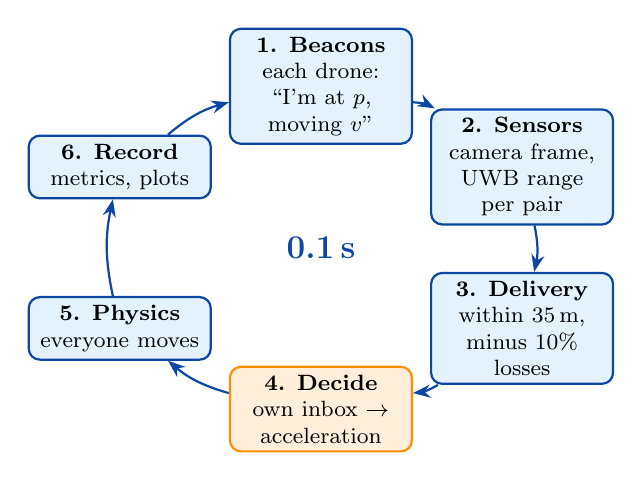
\begin{tikzpicture}[
    tickstep/.style={box, text width=2.1cm, font=\footnotesize, inner sep=3pt},
    ]
  \def\rx{2.95} \def\ry{2.05}
  \node[tickstep] (n1) at (90:{\rx} and {\ry})  {\textbf{1. Beacons}\\ each drone: ``I'm at $p$, moving $v$''};
  \node[tickstep] (n2) at (30:{\rx} and {\ry})  {\textbf{2. Sensors}\\ camera frame, UWB range per pair};
  \node[tickstep] (n3) at (-30:{\rx} and {\ry}) {\textbf{3. Delivery}\\ within 35\,m, minus 10\% losses};
  \node[tickstep, draw=highlight, fill=highlight!15] (n4) at (-90:{\rx} and {\ry}) {\textbf{4. Decide}\\ own inbox $\rightarrow$ acceleration};
  \node[tickstep] (n5) at (-150:{\rx} and {\ry}) {\textbf{5. Physics}\\ everyone moves};
  \node[tickstep] (n6) at (150:{\rx} and {\ry})  {\textbf{6. Record}\\ metrics, plots};
  \node[font=\large\bfseries, text=primary, align=center] at (0,0) {0.1\,s};
  \foreach \a/\b in {n1/n2, n2/n3, n3/n4, n4/n5, n5/n6, n6/n1}
    \draw[arr] (\a) to[bend left=12] (\b);
\end{tikzpicture}
\end{column}
\end{columns}
\end{frame}

% ── Communication ────────────────────────────────────
\begin{frame}{How Drones Talk}
\begin{columns}[T]
\begin{column}{0.48\textwidth}
\textbf{Who hears whom}
\begin{itemize}\small
  \item Drone $i$ hears $j$ if within 35\,m \textbf{and} the packet survives (90\%)
  % \item Losses are independent per direction, so the network is a \textbf{directed graph}
  % \item \textbf{Re-query}: a drone waiting for information gets a second, independent chance next tick
\end{itemize}
\vspace{0.3em}
\textbf{What the liar can and can't do}
\begin{itemize}\small
  \item Every message is stamped with its true sender (models digital signatures)
  \item It \yes\ can lie about itself and refuse to forward others' messages
  \item It \no\ cannot impersonate another drone or tell different neighbours different stories
\end{itemize}
\end{column}
\begin{column}{0.48\textwidth}
\begin{block}{Beacons: short status, direct neighbours}
\small Sent every tick, so \textbf{silence is informative}: 9 silent ticks $\Rightarrow$ out of range ($0.1^9$, one in a billion). This is the only probabilistic assumption in the safety reasoning.
\end{block}
\vspace{0.2em}
\begin{block}{Events: news for the whole fleet}
\small Spread by \textbf{gossip}: each drone forwards new events once, one hop per tick, ignoring duplicates. Capped at 64 per drone per tick, in priority order:\\
\textbf{accusations} $>$ survivors $>$ coverage $>$ terrain
\end{block}
\end{column}
\end{columns}
\end{frame}

% ── Memory and planning ──────────────────────────────
\begin{frame}{How a Drone Remembers and Plans}
\begin{columns}[T]
\begin{column}{0.48\textwidth}
\textbf{\color{primary}Every claim remembers who vouched}\\[0.3em]
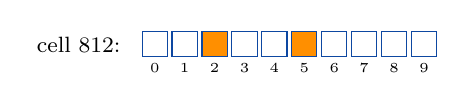
\begin{tikzpicture}
  \node[font=\footnotesize, anchor=east] at (-0.15,0.15) {cell 812:};
  \foreach \i in {0,...,9} {
    \ifnum\i=2 \def\cellc{highlight}\else\ifnum\i=5 \def\cellc{highlight}\else\def\cellc{white}\fi\fi
    \draw[primary, fill=\cellc] (\i*0.38,0) rectangle ++(0.32,0.32);
    \node[font=\tiny] at (\i*0.38+0.16,-0.15) {\i};
  }
\end{tikzpicture}\\[0.1em]
{\small Searched \emph{according to drones 2 and 5} (a 64-bit mask). Liar caught $\Rightarrow$ claims resting only on it go back to \textbf{unsearched}}

\vspace{0.8em}
\textbf{\color{primary}Route planning}\\[0.2em]
{\small Dijkstra on a 2\,m grid of known-free cells; no corner-clipping diagonals; path simplified into straight segments}
\end{column}
\begin{column}{0.48\textwidth}
\textbf{\color{primary}Terrain as ranges, not guesses}\\[0.3em]
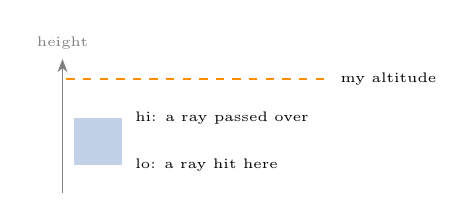
\begin{tikzpicture}
  \draw[gray, -{Stealth}] (0,0) -- (0,1.7) node[above, font=\tiny] {height};
  \fill[primary!25] (0.15,0.35) rectangle (0.75,0.95);
  \node[font=\tiny, anchor=west] at (0.8,0.35) {lo: a ray hit here};
  \node[font=\tiny, anchor=west] at (0.8,0.95) {hi: a ray passed over};
  \draw[highlight, thick, dashed] (0.05,1.45) -- (3.4,1.45) node[right, font=\tiny, text=black] {my altitude};
\end{tikzpicture}\\[0.1em]
{\small Starts at $[0,\infty)$. Safe only if $\mathit{hi}$ + margin $<$ altitude, so unknown squares are \textbf{never} safe}

\vspace{0.8em}
\textbf{\color{primary}Dividing the work: geodesic Voronoi}\\[0.2em]
{\small Claim the cells closest \emph{by flight path}, recomputed every second; idle drones steal work; a caught liar is dropped}
\end{column}
\end{columns}
\end{frame}

% ── Mission flow ─────────────────────────────────────
\begin{frame}{What a Drone Does Over a Mission}
\centering
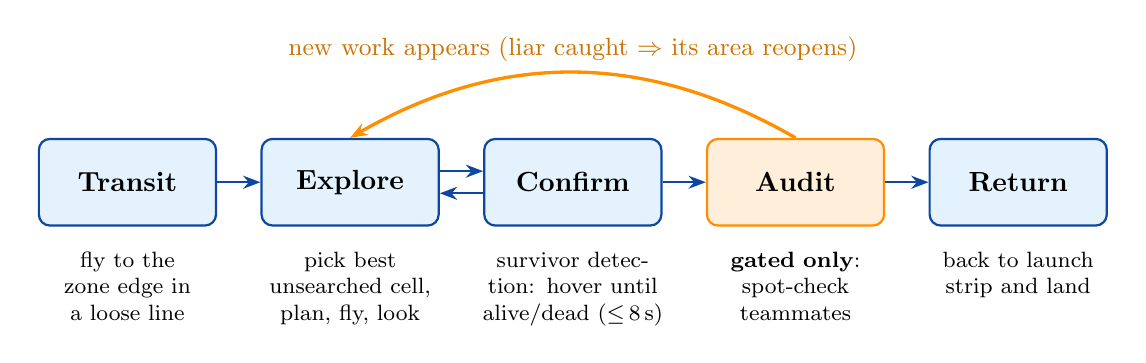
\begin{tikzpicture}[
    node distance=0.55cm,
    mode/.style={box, font=\normalsize\bfseries, minimum width=2.25cm, minimum height=1.1cm},
    desc/.style={font=\footnotesize, text width=2.3cm, align=center, below=0.2cm},
    ]
  \node[mode] (t) {Transit};
  \node[mode, right=of t] (e) {Explore};
  \node[mode, right=of e] (c) {Confirm};
  \node[mode, draw=highlight, fill=highlight!15, right=of c] (a) {Audit};
  \node[mode, right=of a] (r) {Return};
  \node[desc] at (t.south) {fly to the zone edge in a loose line};
  \node[desc] at (e.south) {pick best unsearched cell, plan, fly, look};
  \node[desc] at (c.south) {survivor detection: hover until alive/dead ($\le$\,8\,s)};
  \node[desc] at (a.south) {\textbf{gated only}: spot-check teammates};
  \node[desc] at (r.south) {back to launch strip and land};
  \draw[arr] (t) -- (e);
  \draw[arr] ([yshift=4pt]e.east) -- ([yshift=4pt]c.west);
  \draw[arr] ([yshift=-4pt]c.west) -- ([yshift=-4pt]e.east);
  \draw[arr] (c) -- (a);
  \draw[arr] (a) -- (r);
  \draw[arr, highlight, very thick] (a.north) to[bend right=30]
     node[above, font=\small, text=highlight!80!black] {new work appears (liar caught $\Rightarrow$ its area reopens)} (e.north);
\end{tikzpicture}

\vspace{1.4em}
\small The re-sweep needs no special code: reopened cells simply send drones back to \textbf{Explore}.

\note[item]{Audit: once its own work looks done, a gated drone re-checks a random $q = 10\%$ of each teammate's ``searched'' cells that nobody else has looked at.}
\note[item]{Uniform random sampling makes it meaningful: a hidden survivor in a falsely claimed cell is caught with probability at least about $q$, whatever the liar chose.}
\note[item]{$q$ is the caution knob: raise it to catch more lies, at the cost of finishing later.}
\end{frame}

% =====================================================
\section{Naive Approach}

% ── Naive approach ───────────────────────────────────
\begin{frame}{Naive Approach: Believe Every Claim}
\begin{columns}[c]
\begin{column}{0.52\textwidth}
\textbf{What a naive drone does with what it hears}\\[0.4em]
\footnotesize
\renewcommand{\arraystretch}{1.3}
\begin{tabular}{@{}p{0.6\linewidth} p{0.36\linewidth}@{}}
\toprule
\textbf{Claim} & \textbf{Naive drone} \\
\midrule
``I swept these cells, nobody there'' & \textcolor{bad}{accepts} \\
``This airspace is free''             & \textcolor{bad}{accepts} \\
``Survivor here''                     & \textcolor{bad}{accepts} \\
``I am at position $p$''              & \textcolor{bad}{accepts}, avoids it \\
Numbers (positions, progress)         & W-MSR average \\
\bottomrule
\end{tabular}
\end{column}
\begin{column}{0.44\textwidth}
\begin{itemize}
  \item Same code, sensors and maps as gated: only the \textbf{trust rule} differs
  \item Trusts anyone \emph{not yet proven} a liar, but \textbf{never checks}, so that means trusts everyone forever
  \item \textbf{No} lie checks, \textbf{no} audits, \textbf{no} safety gate
  \item Done when \emph{believed} coverage is complete
\end{itemize}
\vspace{0.3em}
\begin{block}{W-MSR in one line}
\small Drop the $F$ highest and $F$ lowest neighbour values, average the rest: the result stays within the honest range
\end{block}
\end{column}
\end{columns}
\end{frame}

% ── The liar ─────────────────────────────────────────
\begin{frame}{The Liar Drone}
\centering
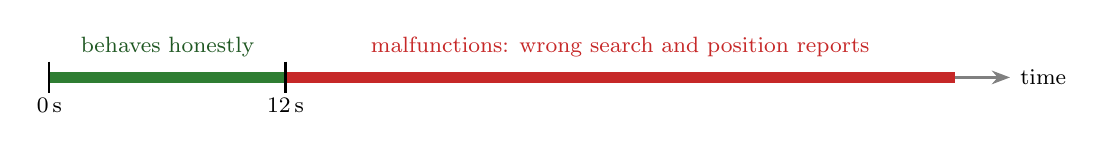
\begin{tikzpicture}
  \draw[good, line width=4pt] (0,0) -- (3,0);
  \draw[bad, line width=4pt] (3,0) -- (11.5,0);
  \draw[-{Stealth}, thick, gray] (11.5,0) -- (12.2,0) node[right, font=\footnotesize, text=black] {time};
  \foreach \x/\l in {0/0\,s, 3/12\,s} {
    \draw[thick] (\x,0.2) -- (\x,-0.2);
    \node[below=4pt, font=\footnotesize] at (\x,0) {\l};
  }
  \node[above=4pt, font=\footnotesize, text=good!70!black] at (1.5,0) {behaves honestly};
  \node[above=4pt, font=\footnotesize, text=bad] at (7.25,0) {malfunctions: wrong search and position reports};
\end{tikzpicture}

\vspace{1em}
\raggedright
\begin{columns}[T]
\begin{column}{0.48\textwidth}
\begin{block}{Fakes its search}
Stops searching and hovers, broadcasting ``searched, nobody here'' for its target corner. It \textbf{never reports} any survivor it sees.
\end{block}
\end{column}
\begin{column}{0.48\textwidth}
\begin{block}{Fakes its position}
Broadcasts a fake search pattern over the corner. Since listeners measure true distance by UWB.
\end{block}
\end{column}
\end{columns}

\vspace{0.8em}
\centering
\small A \textbf{malfunction}, not an attack: same code and sensors as an honest drone, cannot fake a UWB distance or forge others' messages
\end{frame}

% ── Where naive fails ────────────────────────────────
\begin{frame}{Where the Naive Approach Fails}
\begin{columns}[T]
\begin{column}{0.48\textwidth}
\centering
{\color{bad}\Large\bfseries 1}\quad\textbf{A careful liar is never trimmed}\\[0.2em]
{\small It keeps its numbers inside the honest range, so W-MSR never filters it out}
\end{column}
\begin{column}{0.48\textwidth}
\centering
{\color{bad}\Large\bfseries 2}\quad\textbf{Claims aren't numbers}\\[0.2em]
{\small ``I searched this block'' has nothing to average, so filtering can't help}
\end{column}
\end{columns}

\vspace{1.6em}
\centering
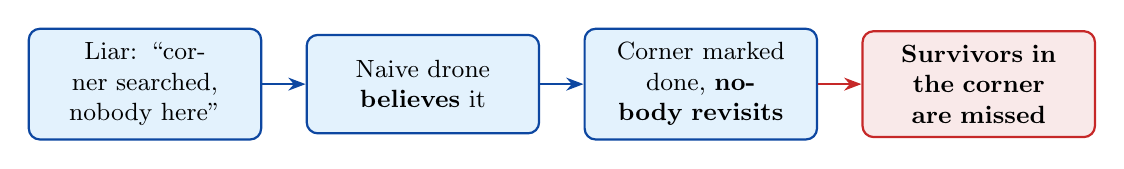
\begin{tikzpicture}[node distance=0.55cm, every node/.style={text width=2.6cm, minimum height=1.25cm}]
  \node[box] (l) {Liar: ``corner searched, nobody here''};
  \node[box, right=of l] (b) {Naive drone \textbf{believes} it};
  \node[box, right=of b] (d) {Corner marked done, \textbf{nobody revisits}};
  \node[badbox] (m) [right=of d] {\textbf{Survivors in the corner are missed}};
  \draw[arr] (l) -- (b); \draw[arr] (b) -- (d); \draw[arr, bad] (d) -- (m);
\end{tikzpicture}
\end{frame}

% =====================================================
\section{Our Approach: Gated}

% ── Gated idea ───────────────────────────────────────
\begin{frame}{Our Approach: Separate Knowing from Believing}
\begin{columns}[c]
\begin{column}{0.42\textwidth}
\begin{itemize}
  \item \textbf{Belief}: someone not yet proven a liar said it $\rightarrow$ used to \textbf{share out work}
  \item \textbf{Knowledge}: true in \emph{every} possible world about who the liar is $\rightarrow$ needed for \textbf{risky actions}: flying into a gap, declaring an area searched
  \item Liar identified $\Rightarrow$ every other claim becomes knowledge
\end{itemize}
\vspace{0.3em}
{\small Believed $-$ known coverage = \alert{the ignorance} we measure}
\end{column}
\begin{column}{0.56\textwidth}
\centering
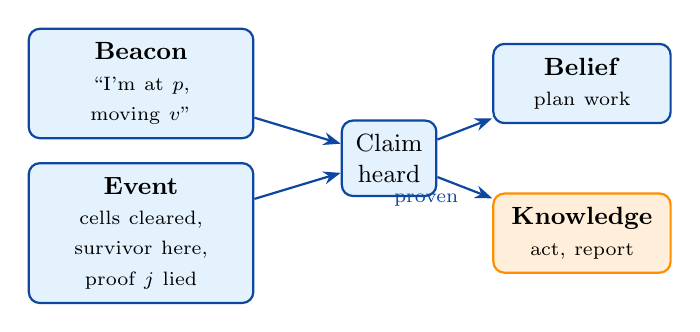
\begin{tikzpicture}[node distance=0.5cm]
  \node[box, text width=2.5cm] (bc) at (0,0.95) {\textbf{Beacon}\\{\scriptsize ``I'm at $p$, moving $v$''}};
  \node[box, text width=2.5cm] (ev) at (0,-0.95) {\textbf{Event}\\{\scriptsize cells cleared, survivor here, proof $j$ lied}};
  \node[box] (c) at (3.15,0) {Claim\\ heard};
  \node[box, text width=1.9cm] (b) at (5.6,0.95) {\textbf{Belief}\\{\scriptsize plan work}};
  \node[hl, text width=1.9cm] (k) at (5.6,-0.95) {\textbf{Knowledge}\\{\scriptsize act, report}};
  \draw[arr] (bc) -- (c); \draw[arr] (ev) -- (c);
  \draw[arr] (c) -- (b);
  \draw[arr] (c) -- node[below left=-2pt, font=\scriptsize] {proven} (k);
\end{tikzpicture}

\vspace{0.6em}
\footnotesize
\renewcommand{\arraystretch}{1.2}
\begin{tabular}{@{}l p{0.72\linewidth}@{}}
\textbf{Beacon} & checked against UWB range, camera and speed limits \\
\textbf{Event}  & stored with \emph{who vouched}, judged by who might be lying \\
\end{tabular}
\end{column}
\end{columns}
\end{frame}

% ── Catching lies ────────────────────────────────────
\begin{frame}{Catching Lies}
\centering\small
\renewcommand{\arraystretch}{1.22}
\begin{tabular}{@{}c l p{8.8cm}@{}}
\multicolumn{3}{@{}l}{\small\color{primary}\textbf{Proof: these name exactly who lied}} \\
\rbadge{R1} & \textbf{Distance} & claimed position doesn't match the distance I measured \\
\rbadge{R2} & \textbf{Speed}    & claimed movement is faster than any drone can fly \\
\rbadge{R3} & \textbf{Radio}    & claims to be out of range, yet I can hear it \\
\rbadge{R4} & \textbf{Camera}   & claims a spot my camera shows is empty \\
\rbadge{R5} & \textbf{Audit}    & I found a survivor in a cell it called empty \\[0.1em]
\multicolumn{3}{@{}l}{\small\color{highlight!80!black}\textbf{Hint: this only narrows it down}} \\
\rbadge[highlight]{R6} & \textbf{Shared distance} & another drone's distance contradicts it: \emph{one of the two} lied \\
\end{tabular}

\vspace{0.6em}
\begin{block}{Design rule}
\centering An honest drone can \textbf{never} fail a check $\Rightarrow$ \textbf{no innocent drone is ever accused}
\end{block}
\end{frame}

% ── Safety gate ──────────────────────────────────────
\begin{frame}{The Safety Gate: ``Do I \emph{Know} This Move Is Safe?''}
\begin{columns}[c]
\begin{column}{0.48\textwidth}
\centering
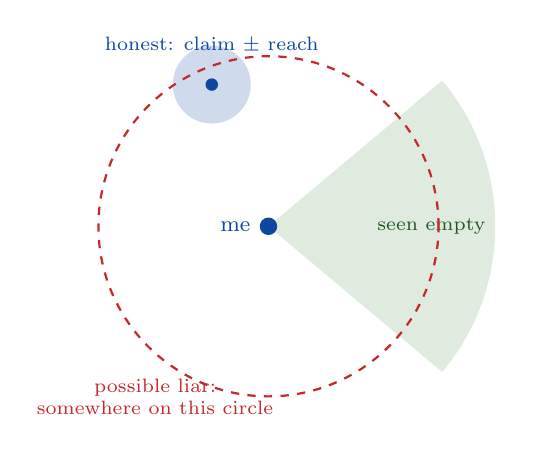
\begin{tikzpicture}[scale=0.9]
  % camera seen-empty wedge
  \fill[good!15] (0,0) -- (40:3.2) arc (40:-40:3.2) -- cycle;
  \node[font=\scriptsize, good!70!black] at (2.3,0) {seen empty};
  % me
  \fill[primary] (0,0) circle (3.5pt) node[left=3pt, font=\footnotesize] {me};
  % honest neighbour zone
  \fill[primary!20] (-0.8,2.0) circle (0.55);
  \fill[primary] (-0.8,2.0) circle (2.5pt) node[above=8pt, font=\scriptsize] {honest: claim $\pm$ reach};
  % possible liar sphere
  \draw[bad, thick, dashed] (0,0) circle (2.4);
  \node[font=\scriptsize, bad, align=center] at (-1.6,-2.4) {possible liar:\\ somewhere on this circle};
\end{tikzpicture}
\end{column}
\begin{column}{0.48\textwidth}
\begin{itemize}
  \item \textbf{Maybe honest}: stay $\ge$1\,m from where it could be
  \item \textbf{Maybe liar}: its claim is ignored, but its \emph{measured} distance isn't. That circle must be far away or \textbf{seen empty}
  \item Not sure $\Rightarrow$ \textbf{brake and re-query}
\end{itemize}
\vspace{0.4em}
{\footnotesize Deadlock $>$1\,s: higher id backs off \textbullet{} $>$3\,s: pick a new target}
\end{column}
\end{columns}
\end{frame}

% ── Naive vs gated ───────────────────────────────────
\begin{frame}{Naive vs.\ Gated}
\centering
\renewcommand{\arraystretch}{1.45}
\begin{tabular}{l c c}
\toprule
 & \textbf{Naive} & \cellcolor{lightbg}\textbf{Gated} \\
\midrule
Acts on                    & anything not yet disproven  & \cellcolor{lightbg} proven facts (knowledge) \\
Combines numbers with      & W-MSR                       & \cellcolor{lightbg} W-MSR, minus proven liars \\
Checks for lies (R1--R6)   & \no                         & \cellcolor{lightbg} \yes \\
Audits teammates           & \no                         & \cellcolor{lightbg} \yes \\
\textbf{Safety gate}       & \no\ trusts claimed positions & \cellcolor{lightbg} \yes\ moves only if \emph{known} safe \\
Liar's claims once caught  & kept forever                & \cellcolor{lightbg} reverted and re-swept \\
\bottomrule
\end{tabular}

\vspace{1em}
Same drone code, same map, same seed: \textbf{any difference is caused by trust}.
\end{frame}

% =====================================================
\section{Live Demo}

% ── Live demo: observations ──────────────────────────
\begin{frame}{Live Demo}
\subhead{Observations from the demo}
\centering
\renewcommand{\arraystretch}{1.35}
\begin{tabular}{l c c}
\toprule
 & \textbf{naive} & \textbf{gated} \\
\midrule
Survivors found     & \textcolor{bad}{\textbf{10 / 16}} & \textcolor{good}{\textbf{16 / 16}} \\
Missed in liar's area & \textcolor{bad}{6} & \textcolor{good}{0} \\
Collisions          & \textcolor{bad}{6} & \textcolor{good}{0} \\
Everyone knows the liar & n/a & $\approx$\,\textbf{13\,s} \\
False accusations   & 0 & 0 \\
\bottomrule
\end{tabular}

\vspace{1em}
\raggedright
\begin{columns}[T]
\begin{column}{0.48\textwidth}
\begin{alertblock}{Naive}
Trusts ``nobody here'' and \textbf{never enters the liar's corner}
\end{alertblock}
\end{column}
\begin{column}{0.48\textwidth}
\begin{block}{Gated}
Catches the liar drone, the corner \textbf{reopens and is re-swept}
\end{block}
\end{column}
\end{columns}
\end{frame}

% =====================================================
\section{Benchmarks}

% ── How the experiments were run ─────────────────────
\begin{frame}{How the Experiments Were Run}
\begin{columns}[c]
\begin{column}{0.56\textwidth}
\centering
\textbf{One parameter at a time}\\[0.8em]
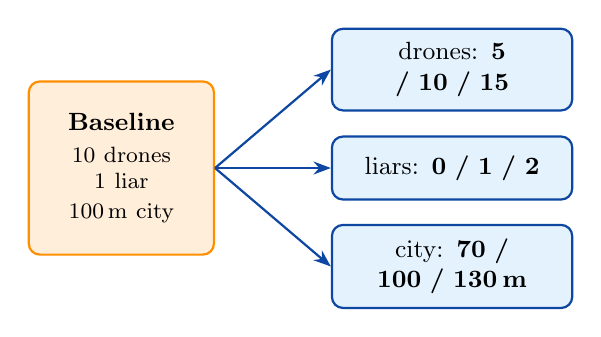
\begin{tikzpicture}[
    vary/.style={box, text width=2.7cm, minimum height=0.8cm, font=\small},
    ]
  \node[hl, text width=2.0cm, minimum height=2.2cm] (base) at (0,0)
     {\textbf{Baseline}\\[2pt]{\footnotesize 10 drones\\ 1 liar\\ 100\,m city}};
  \node[vary] (n) at (4.2, 1.25) {drones: \textbf{5 / 10 / 15}};
  \node[vary] (l) at (4.2, 0)    {liars: \textbf{0 / 1 / 2}};
  \node[vary] (z) at (4.2,-1.25) {city: \textbf{70 / 100 / 130\,m}};
  \foreach \t in {n,l,z} \draw[arr] (base.east) -- (\t.west);
\end{tikzpicture}

\vspace{1em}
\stat{20}{seeds per value} \hfill \stat{7}{settings} \hfill \stat{280}{runs}
\end{column}
\begin{column}{0.40\textwidth}
\begin{enumerate}\small
  \item Each seed is a new district and survivor layout
  \item Naive and gated fly the \textbf{same seed}: same map, liar and noise
  \item 480\,s limit per run
  \item Plots: \textbf{mean of 20 seeds} with 95\% interval (shaded)
\end{enumerate}
\vspace{0.4em}
{\footnotesize Here naive also runs the safety check (believing everyone), so the fleets differ \textbf{only in trust}.}
\end{column}
\end{columns}
\end{frame}

% ── Survivors found ──────────────────────────────────
\begin{frame}{Benchmark: Survivors Found}
\centering
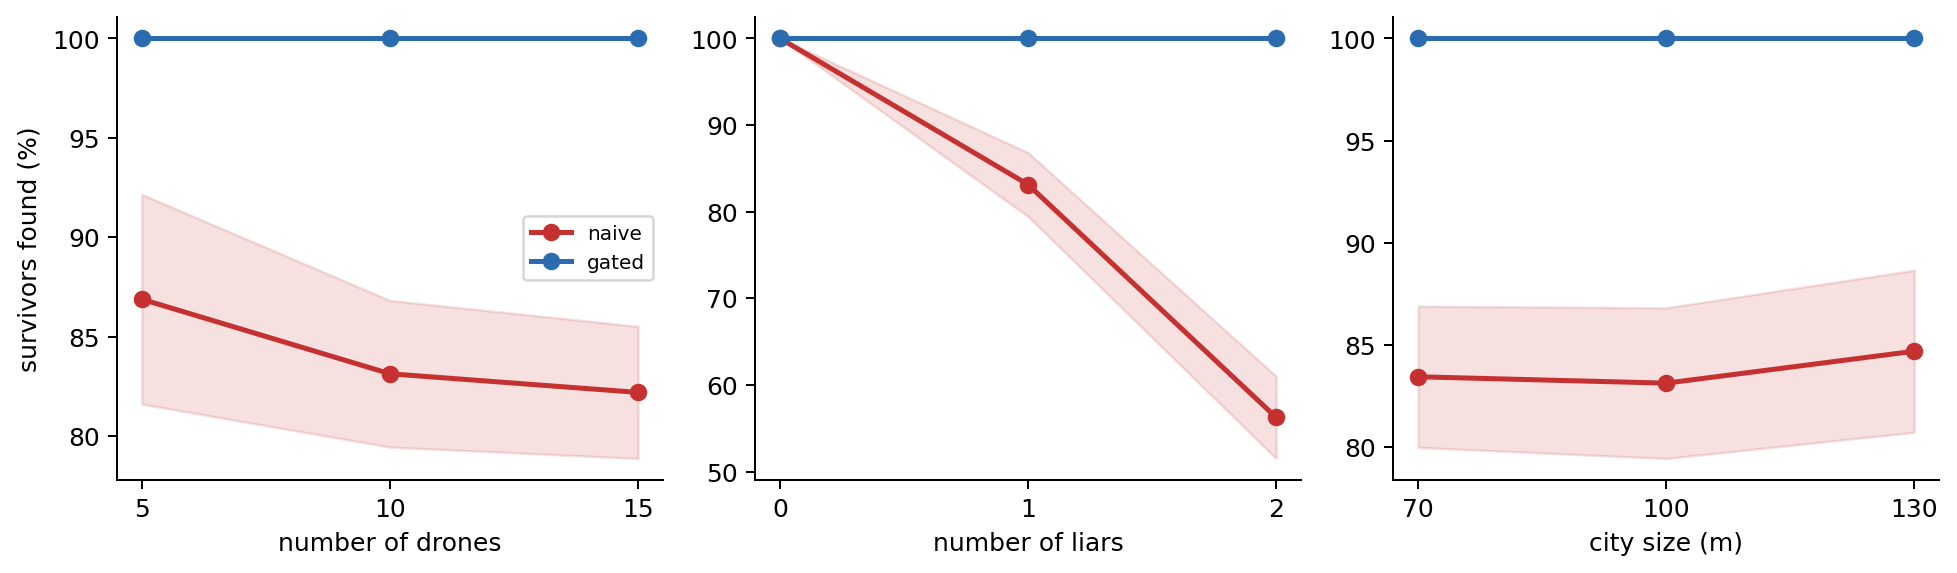
\includegraphics[width=\linewidth,height=4.3cm,keepaspectratio]{figures/sweep_found.png}

\vspace{0.6em}
\begin{columns}[T]
\begin{column}{0.32\textwidth}
\centering\stat{100\%}{gated, in all 140 runs}
\end{column}
\begin{column}{0.32\textwidth}
\centering\stat{83\%}{naive, 1 liar (worst run 69\%)}
\end{column}
\begin{column}{0.32\textwidth}
\centering\stat{56\%}{naive, 2 liars (worst run 44\%)}
\end{column}
\end{columns}

\vspace{0.5em}
\footnotesize Naive is perfect only when nobody lies \textbullet{} gap significant wherever a liar is present ($p < 0.002$) \textbullet{} liar caught in every gated run, 0 false accusations
\end{frame}

% ── Completion time ──────────────────────────────────
\begin{frame}{Benchmark: Completion Time}
\centering
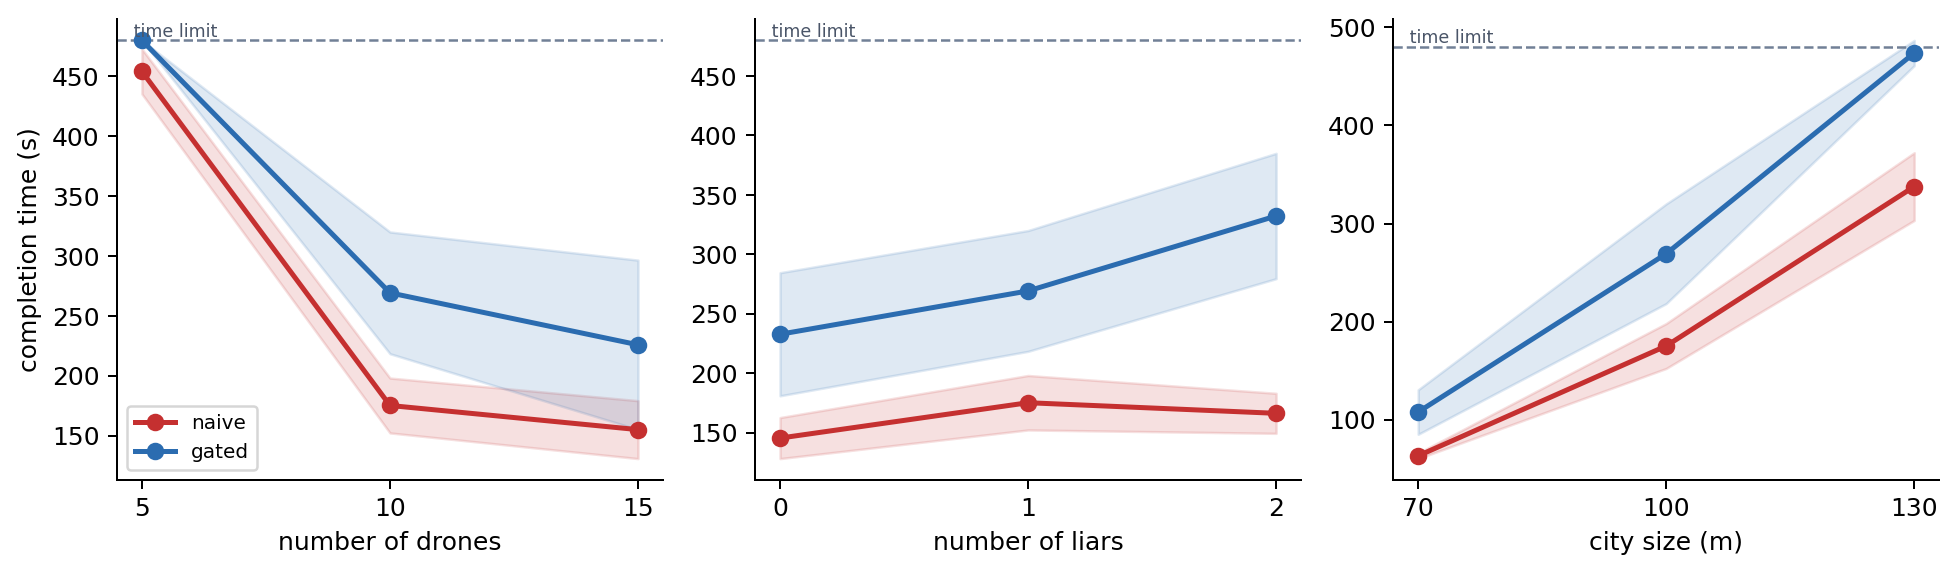
\includegraphics[width=\linewidth,height=4.3cm,keepaspectratio]{figures/sweep_time.png}

\vspace{0.6em}
\begin{columns}[T]
\begin{column}{0.32\textwidth}
\centering\stat{269 vs 175\,s}{gated vs naive at baseline}
\end{column}
\begin{column}{0.32\textwidth}
\centering\stat{+87\,s}{cost of caution with no liar}
\end{column}
\begin{column}{0.32\textwidth}
\centering\stat{480\,s}{gated hits the limit: 5 drones, 130\,m city}
\end{column}
\end{columns}

\vspace{0.5em}
\footnotesize Caution costs time, not lives \textbullet{} more drones shorten the mission for both fleets
\end{frame}

% =====================================================
\section{Limitations}

% ── Limitations ──────────────────────────────────────
\begin{frame}{Limitations}
\begin{columns}[T]
\begin{column}{0.48\textwidth}
\begin{block}{Performance}
\begin{itemize}\small
  \item \textbf{Caution costs time}: about +90\,s at baseline, even with no liar
  \item \textbf{Small fleets, large cities}: gated rarely finishes within 480\,s (5 drones, 130\,m)
  \item \textbf{Coverage-only liar} (flies its true position): caught only by audits, 13/20 runs, median 44\,s
\end{itemize}
\end{block}
\end{column}
\begin{column}{0.48\textwidth}
\begin{block}{Design and model}
\begin{itemize}\small
  \item ``Done'' uses belief + audits; \emph{known}-cleared coverage is reported, not required
  \item Safety gate skips a possible liar with no range reading that tick (relies on the silence rule)
  \item Coverage claims impossible from the liar's true path aren't used as proof yet
  \item Assumes signed messages, no equivocation, range noise $\le$\,0.2\,m, static 2.5D terrain, point drones, no wind
\end{itemize}
\end{block}
\end{column}
\end{columns}
\end{frame}

% % =====================================================
% \section{Contributions}

% % % ── Individual contributions ─────────────────────────
% % \begin{frame}{Individual Contributions}
% % \centering
% % \renewcommand{\arraystretch}{1.5}
% % \begin{tabular}{@{}l l l@{}}
% % \toprule
% % \textbf{Member} & \textbf{Role} & \textbf{Key parts} \\
% % \midrule
% % Rithvik Jami              & Simulator and network & tick loop, radio, robustness study,integration \\
% % Praneeth Chamarthy        & Mission and planning  & modes, W-MSR, maps, Voronoi \\
% % Muvvala Sai Ram Suhas     & Epistemic layer       & lie checks, audits, safety gate, liar model \\
% % Jakkala Naga Rohith Kumar & World and analysis    & city and camera,STL,dashboard,benchmarks \\
% % Gona Sanjana              & Supporting study      & survivor localisation \\
% % Prabhu Teja               & Demo support          & scenario and seed set-up \\
% % \bottomrule
% % \end{tabular}

% \vspace{0.8em}
% {\footnotesize\color{gray}Detailed contributions are in the report.}
% \end{frame}

% ── Thank You ────────────────────────────────────────
\begin{frame}[standout]
    \Huge Thank You\\[0.5em]
    \normalsize Questions?
\end{frame}

\end{document}
